This \cgal\ package provides functions to compute global informations
on the shape of a set of 2D or 3D objects such as points. It provides the computation of bounding boxes, centroids of point sets, barycenters of weighted point sets, as well as linear least squares fitting.

Linear least squares fitting approximates a set of objects by a linear
sub-space such as a line or a plane. Formally, given a set of points in $R^d$, linear least squares fitting amounts
to find the linear sub-space of $R^d$ which minimizes the sum of squared
distances from the points to their projection onto this linear sub-space. This
problem is equivalent to search for the linear sub-space which maximizes the
variance of projected points, the latter being obtained by eigen decomposition
of the covariance matrix. Eigenvectors corresponding to large eigenvalues are
the directions in which the data has strong component, or equivalently large
variance. If eigenvalues are the same there is no preferable sub-space.
This package implements the linear least squares fitting for
several objects of a \cgal\ 2D or 3D kernel: the best fit 2D line for 2D
point sets, and the best fit 3D line or plane for point and
triangle sets. The object sets are specified by iterator ranges of
containers.

\begin{center}
    \label{PCA}
    % Image
    \begin{ccTexOnly}
      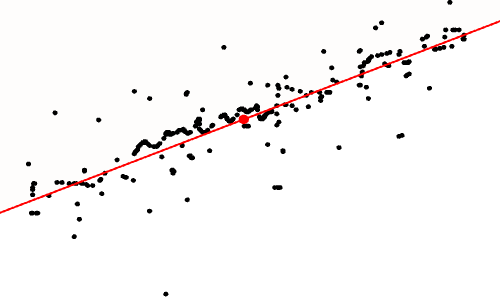
\includegraphics[width=0.45\textwidth]{Principal_component_analysis/fit_2d}
    \end{ccTexOnly}
    \begin{ccHtmlOnly}
        <img width="45%" border=0 src="./fit_2d.png"><P>
    \end{ccHtmlOnly}
    % Title
    \begin{figure}[h]
        \caption{Fitting a line to a 2D point set.}
    \end{figure}
\end{center}

